\documentclass{article}
\usepackage{fancyhdr}
\usepackage{extramarks}
\usepackage{amsmath}
\usepackage{amsthm}
\usepackage{amsfonts}
\usepackage{tikz}
\usepackage[plain]{algorithm}
\usepackage{algpseudocode}

\begin{document}
\author{Chuan Lu}
\title{BIOS:7600 Homework 2}
\maketitle

\medskip

\begin{enumerate}

\item Derive the relationship between FDR and local FDR.
$$
\mathbb{E}(\text{fdr}(z)|z\in\mathcal{Z}) = \mathbb{E}(\mathbb{P}(H_0|z)|z\in\mathcal{Z}) = \mathbb{P}(H_0|z\in\mathcal{Z}) = \mathbb{E}(A_Z/R_Z) = \text{Fdr}(\mathcal{Z}).
$$

\item Show that if $cX \sim \chi_\nu^2 $, then $X \sim \text{Gamma}(\frac{\nu}{2}, \frac{c}{2})$.

By CDF of the $\chi^2 $ distribution,
$$
\mathbb{P}(cX < x) = \frac{\gamma(\frac{\nu}{2}, \frac{x}{2})}{\Gamma(\frac{\nu}{2})}.
$$
Hence
$$
F_X(x) = \mathbb{P}(X < x) = \frac{\gamma(\frac{\nu}{2}, \frac{cx}{2})}{\Gamma(\frac{\nu}{2})} \sim \text{Gamma}(\frac{\nu}{2}, \frac{c}{2}).
$$

\item State the answer.
\begin{enumerate}
\item In BH, the $q$-value with $z = 0$.

$q = 0.5$.

\item What is the $q$-value with $z = 0$ if estimate $\pi_0 $?


\item For GMM, what's the range of fdr for $z = 0$?

$(0, \frac{1}{2})$.

\item For GMM, what's the range of fsr for $z\to 0^+ $?


\end{enumerate}

\item 

(I wonder how to get the $p$-values by $z$-values. I suppose here to use two-tail test, but I don't know if it's correct.)

\begin{table}[]
\centering
\begin{tabular}{lllll}
\hline
group & mean      & std        &  &  \\
\hline
1     & 0.1971197 & 0.08333976 &  &  \\
\hline
2     & 0.198178  & 0.04258965 &  &  \\
\hline
      &           &            &  & 
\end{tabular}
\end{table}

The histograms of the FDRs are shown as follows. The left one is for the first set of $Z$-values, and the right one is for the second set. We can see that correlations do not have a large influence on the mean of FDRs, but result in a larger standard deviation.

\begin{figure}[h]
\centering
\vbox{
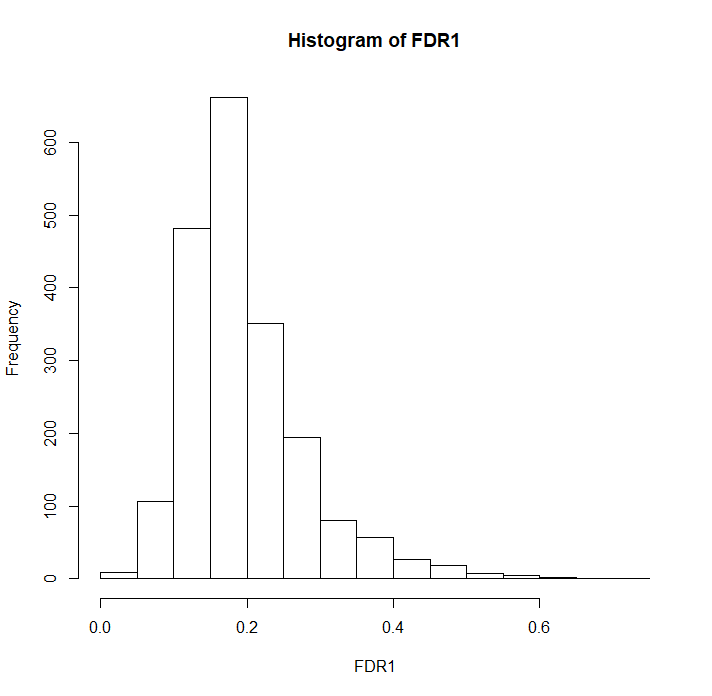
\includegraphics[scale=0.3]{problem4_FDR1.png}
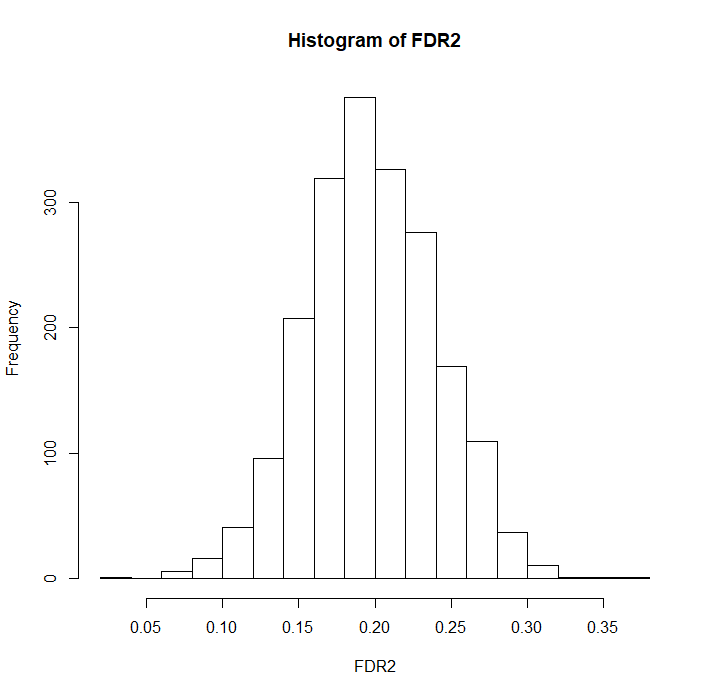
\includegraphics[scale=0.3]{problem4_FDR2.png}
}
\end{figure}

\item

\end{enumerate}


\end{document}